\def\year{2016}\relax
\documentclass[letterpaper]{article}
\usepackage{aaai16}
\usepackage{times}
\usepackage{helvet}
\usepackage{courier}

\usepackage{graphicx}
\usepackage{epstopdf}
\usepackage[noend]{algorithmic}
\usepackage{algorithm}
\usepackage{amsmath}
\usepackage{amsfonts}
\usepackage{multirow}



\frenchspacing
\setlength{\pdfpagewidth}{8.5in}
\setlength{\pdfpageheight}{11in}

\usepackage{amsmath,amssymb}
\newtheorem{theorem}{Theorem}
\newtheorem{lemma}{Lemma}
\newtheorem{corollary}{Corollary}
\newtheorem{example}{Example}
\newtheorem{definition}{Definition}
\newenvironment{proof}{\par\noindent{\em Proof.}}{\hfill $\Box$\medskip}
\def\minimize{\mathop{\mbox{\bf minimize}}}
\def\maximize{\mathop{\mbox{\bf maximize}}}
\def\subjectto{\mathop{\mbox{\bf subject to}}}
\DeclareMathOperator*{\argmin}{\arg\!\min}
\DeclareMathOperator*{\argmax}{\arg\!\max}
\newcommand{\GHS}{\mbox{\tt GHS}}
\newcommand{\CS}{\mbox{\tt CS}}
\newcommand{\roni}[1]{\mbox{\tt RONI: #1}}
\renewcommand{\algorithmicrequire}{\textbf{Input:}}
\renewcommand{\algorithmicensure}{\textbf{Output:}}


\setcounter{secnumdepth}{0}
\begin{document}
\title{Searching with a Corrupted Heuristic}

\author
{Levi H.S. Lelis\\Universidade Federal de Vicosa \\ levi.lelis@ufv.br \And
Richard Valenzano\\University of Toronto\\rvalenzano@cs.toronto.edu \AND
Gabriel Nazar\\Universidade Federal do Rio Grande do Sul \\ glnazar@inf.ufrgs.br
\And
Roni Stern\\Ben Gurion University of the Negev\\roni.stern@gmail.com
}

\maketitle
\begin{abstract}
Memory-based heuristics are a popular and effective class of admissible heuristic functions.  However, corruptions to memory they use may cause these heuristics to become inadmissible.  Corruption can be caused by the physical environment due to radiation and network errors, or it can be introduced voluntarily as a way to decrease energy consumption. We introduce memory error correction schemes that do not require additional memory and exploit knowledge about the behavior of consistent heuristic functions.  This is in contrast with error correcting code approaches which can limit the amount of corruption but at the cost of additional energy and memory consumption. Search algorithms using our methods are bounded-suboptimal and are guaranteed to find a solution if one exists. Moreover, our methods are resilient to any number of memory errors that may occur. An experimental evaluation is also provided to demonstrate the applicability of our approach.
\end{abstract}

\section{Introduction}

Memory-based heuristics such as pattern databases~\cite{culberson1998patternDatabases,Edelkamp01planningwith} and differential heuristics~\cite{stutervant2009memoryBased} are a popular and effective way of guiding search algorithms like A*~\cite{hart1968aFormalBasis} and Iterative-Deepening A* (IDA*)~\cite{korf85} when solving state-space search problems.

For example, a pattern database (PDB) is a pre-computed lookup table that contains the optimal solution costs for states in an abstracted and smaller version of the original state space. The entries of the lookup table serve as heuristic estimates for states in the original state space.
PDBs frequently require a few GBs of memory which must be stored in fast-access memories such as dynamic RAMs (DRAMs). This is because search algorithms consult the PDB for every node generated during search. And since memories play an important role in the overall energy consumption of systems \cite{5695550}, the means to store PDBs are not only crucial for performance, but also for energy consumption.

Energy has become a major constraint not only for embedded systems but also in clusters and server-farms~\cite{Cameron2005}. One prospective approach to reduce energy consumption is approximate computing. Approximate computing comprises a broad set of mechanisms that generally trade precision for energy efficiency. For example, computational precision can be traded for energy efficiency by reducing the hardware supply voltage
\cite{974895} or by designing low-power arithmetic circuits with approximate outputs \cite{5993675}. These approaches can also reduce energy consumption when using specific memory technology. For example, SRAM cells can have their supply voltage reduced \cite{5686921}, while DRAM can have their refresh frequency reduced \cite{Liu:2011:FSD:1950365.1950391}. %In this paper we focus on memory-based approaches. %See the work of Venkataramani \textit{et al.} \shortcite{Venkataramani:2015:ACQ:2744769.2751163} for a comprehensive review on approximate computing.

The general tradeoff when using memory-based approximate computing schemes is that the larger the data and the greater the acceptable degree of imprecision, the more energy can be saved. Since memory-based heuristics like PDBs are typically very large, they are excellent candidates for approximation. However, unchecked errors in the PDB can lead to severely suboptimal solutions, which can be catastrophic for some applications. %Performance, in terms of execution time, can also be greatly affected.

In addition to approximate computing schemes, memory corruption can also be caused by other phenomena.
For example, radioactive particles and electrical noise are a concern not only in spaceborne applications~\cite{Wagstaff_kmeansin}, but also in applications running in large data centers~\cite{7266869}. The standard mechanism to mitigate memory errors in these scenarios are Error Correcting Codes (ECC), which incur additional memory and energy costs. %are not without costs and, as such, their partial application to memories also allows trading precision for energy efficiency, as investigated in \cite{Luo:2014:CAM:2671853.2672438}. %Applications operating in harsh environments, such as spaceborne systems, typically face stringent and conflicting energy and dependability constraints, and therefore can also benefit from such approaches \cite{6517720}.
Memory corruptions may also occur due to network errors in case of a distributed-memory architecture.


In this paper we introduce algorithms to handle memory errors in memory-based heuristics. % with the goal of benefiting from the energy efficiency provided by approximate computing strategies.
The proposed algorithms are based on IDA* and novel error detection and correction methods. Our algorithms are guaranteed to find a solution if one exists and the cost of the solution they find is no more than three times larger than the problem's optimal solution cost. In contrast with other algorithms that are resilient to memory corruption (see Finocchi et al.~\shortcite{finocchi2007designing} for examples), our methods do not assume an upper bound on the number of memory errors that may occur during search.

Experiments on standard search benchmarks show the advantages of our correction methods in terms of suboptimality. We also show the advantages of our methods over a variety of ECC approaches with respect to memory and energy consumption. For example, while our approaches increase in only 5\% the energy and memory consumed by DRAMs, ECCs can have a memory and energy overhead of up to 40\%.

\section{Selective Reduction of the Refresh Rate}

We begin by reviewing one of the approximate computing schemes used for decreasing the energy usage of a system by allowing for memory corruption. However, existing search techniques are unable to take advantage of such potential savings since they are not designed to handle heuristic corruption. This provides one possible motivation for the investigation performed in this paper. However, it should be noted that our methods are general and can be used to detect and correct errors in memory-based heuristic functions in general.

DRAM is the most common technology used for main memories, mainly due to its high density and performance. DRAM cells require periodic refresh to maintain their stored values, which consists in reading and rewriting the value in all cells. This operation consumes substantial energy. To reduce this consumption, one alternative is to use a technique known as Flikker \cite{Liu:2011:FSD:1950365.1950391} which reduces the refresh frequency in memory regions that hold non-critical data, %This is possible because these frequencies are determined for worst case cells, being overdimensioned for the vast majority of cells. In newer technologies this phenomenon becomes more prominent, as process variability increases the differences between typical and worst case transistors.
while data that cannot withstand corruption is kept in memory that is refreshed at the nominal frequency. %Liu \textit{et al.} \shortcite{Liu:2011:FSD:1950365.1950391} observed that refresh power is substantially reduced up until refresh periods of 1 second (nominal values are usually 64 or 32 microseconds), while introducing approximately one error for every $4\times10^8$ bits. Further reductions in refresh frequency do not provide relevant gains, as other components begin to dominate the overall memory power. This is thus considered to be a near-optimal period for low-refresh regions.

Substantial gains can be obtained when most of the memory can use the low refresh frequency. This property holds when using a linear-space algorithm alongside standard memory-based heuristics. For example, when using PDBs on the standard benchmarks considered in this paper, the PDB corresponds to at least 95\% of entire program memory. For programs with such large low-refresh regions, approximately 33\% reduction in refresh energy consumption can be expected \cite{Liu:2011:FSD:1950365.1950391}.


\section{Problem Definition and Background}





The state-space search task is to find a sequence of \textbf{operators} that will transform  a given \textbf{initial state} $s_{\mathrm{init}}$ into a \textbf{goal state}. Such search problems can be viewed as \textbf{graph-search problems}: the graph $G = (V, E)$ is the \textbf{state-space}, where each vertex corresponds to a state and an edge $(s,s')\in E$ corresponds to having a single operator transform $s$ to $s'$.
A solution is a path in $G$ from $s_{\mathrm{init}}$ to one of a set of \textbf{goal states} $V_{\mathrm{goals}}\subseteq V$. We use $children(s)$ to denote the set of nodes adjacent to $s$, i.e., $children(s) = \{ s' | (s,s') \in E\}$.  When the
set $children(s)$ of a \textbf{parent} state $s$ is constructed, $s$ is said to be \textbf{expanded} and any $s'\in children(s)$ is said to be \textbf{generated}.

State transition operators, and consequently edges, have a cost, denoted by $\kappa(s, s')$. We assume that $\kappa(s, s')$ is non-negative and that the cost of a path of states $\pi$ in $G$ is the sum of the edges along $\pi$. An optimal solution is a least-cost path from $s_{\mathrm{init}}$ to a goal state and the cost of an optimal solution is denoted by $C^*$. For a given state $s$, we use $h^*(s)$ and $g^*(s)$ to denote the cost of an optimal path from $s$ to a goal node and the cost of an optimal path from $s_{\mathrm{init}}$ to $s$, respectively. %This means that $C^* = h^*(s_{\mathrm{init}}) = g^*(s) + h^*(s)$ where $s$ is any node on some optimal solution path $\pi$.
We also assume that all operators are \textbf{reversible} (\textit{ie.} the edges are undirected) and that they have the same cost in both directions.



IDA*~\cite{korf85} uses an \textbf{evaluation function} on nodes to guide its search. The evaluation function used by IDA* is $g(n) + h(n)$, where $g(n)$ is the cost of the path from $s_{init}$ to $n$ and $h(n)$, referred to as the \textbf{heuristic function}, is an estimate of the cost of the path from $n$ to the nearest goal node.
Many heuristic functions---including the PDB heuristics---are \textbf{state-based}.
This means that where $n$ represents path $[s_0, ..., s_k]$, the heuristic  only takes $s_k$ into account and so will always return the same value for any node that ends in $s_k$.
In contrast, \textbf{path-based} heuristics may return different values depending on the path  found to $s_k$. The error correction heuristics we introduce below are path-based.


A key property of IDA* is that any solution found is guaranteed to be optimal if $h$ is \textbf{admissible} \cite{korf85}. A heuristic function is called admissible if $\forall n, h(n) \leq h^*(n)$.




The error detection and correction methods we introduce in this paper use the consistency property of a heuristic function, defined as follows.

\begin{definition}[Consistency]
A heuristic $h$ is said to be consistent on edge $(n,n')$ iff $|h(n) - h(n')| \le \kappa(n,n')$, and consistent on a state-space problem iff it is consistent on every edge in the graph.
\label{def:consistency}
\end{definition}
Notice that this definition corresponds to definition of consistency on undirected graphs, as the definition is somewhat weaker on directed graphs.

In this work we use the following setting. The memory-based heuristic is pre-computed and safely stored in a slow-access reliable memory and is loaded into DRAM
prior to the search, during which errors may occur and accumulate.







\section{Error Detection}


\begin{figure}[t]
\begin{center}
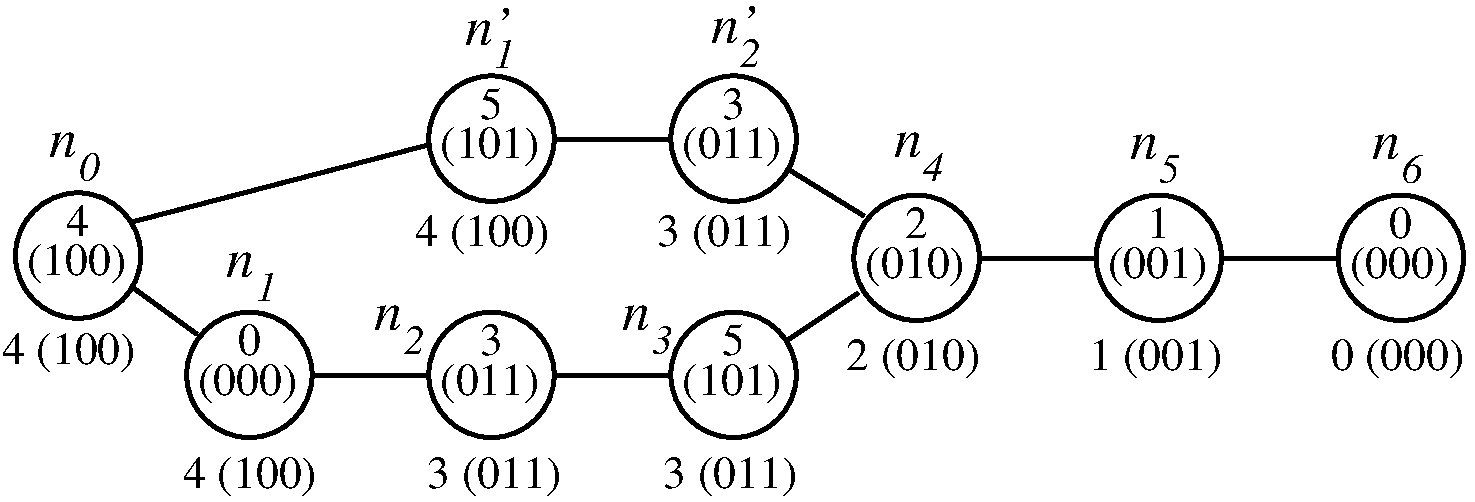
\includegraphics[width=240px]{figures/corruption_example5.pdf}
\caption{An example of a corrupted heuristic.}
\label{fig:corruption_example}
\end{center}
\end{figure}

In this section, we introduce several methods for detecting that a consistent heuristic has been corrupted.
To help introduce these concepts, we will use the unit-cost graph shown in Figure \ref{fig:corruption_example} as a running example.
The uncorrupted heuristic values are shown below each vertex, with the 3-bit binary representation included in parentheses. The heuristic values found after the corruption are shown inside each vertex.

\subsection{Sufficient Detection of Error}

The basic error detection method we will use is based on identifying edges which break the consistency of the heuristic.
If we know the heuristic was initially consistent before corruption occurred, then the existence of an edge $(n, n')$ on which the heuristic is \textit{inconsistent} (\textit{ie.} not consistent) is a clear indication that the heuristic value of either $n$ or $n'$ must have been corrupted.
For example, the corrupted heuristic is inconsistent on edge $(n_0, n_1)$ in Figure \ref{fig:corruption_example}, while the original uncorrupted heuristic is consistent on that edge.
By simply watching for inconsistent edges, we therefore have a simple and sufficient way to detect errors.

Unfortunately, this approach will not necessarily identify all errors.
For example, consider the edge $(n_0, n_1')$ in Figure \ref{fig:corruption_example}.
The heuristic value of $n_1'$ has been corrupted from a value of $4$ to the inadmissible value of $5$.
However, the corrupted heuristic remains consistent on this edge and so this approach will not identify this error.












\subsection{Inadmissibility Detection}

When the heuristic value of a state is decreased, it may increase the time needed to find a solution, but it will not cause suboptimal solutions to be found. It is only when corruption makes a heuristic function inadmissible that we may find suboptimal solutions. Therefore, we may wish to consider techniques that detect when a heuristic value may have become inadmissible. In this section, we consider a lookahead based approach for doing so, prove the correctness of the approach, and consider the issues with this technique. We begin with the following lemma:


\begin{lemma}%[Inadmissible corruption]
\label{lemma:inad_corruption}
If a heuristic $h$ is consistent on edge $(n, c)$ where $h(n)>h^*(n)$, then $h(c) > h^*(c)$ if $c$ is on the optimal path from $n$ to a goal.
\label{lem:inadmissible-corruption}
\end{lemma}
\begin{proof}
Let $c$ be a node on an optimal path from $n$ to a goal.
Thus, $h^*(n)=h^*(c)+\kappa (n,c)$. Since $h$ is consistent on the edge $(n, c)$, then $h(n)\leq h(c)+\kappa(n,c)$. Together with the inadmissibility of $h(n)$ this means the following:
\[ h^*(c)+\kappa(n,c)= h^*(n) < h(n) \leq h(c)+\kappa(n,c) \]
Therefore $h^*(c)<h(c)$ as required.
\end{proof}


This lemma shows consistency on the edge between $n$ and any child $c$ along an optimal path from $n$ means that if $h$ is inadmissible on $n$, then that inadmissibility must have propagated to $n$. Conversely, if $h(c)$ is admissible, $h(n)$ must also be admissible.

Now let us extend the definition of a heuristic being consistent on an edge to define the concept of a heuristic being consistent along a path:

\begin{definition}[Path Consistency]
A heuristic $h$ is said to be consistent along a path of nodes $\pi=[n_0,..,n_k]$ iff $h$ is consistent on every edge along $\pi$.
\end{definition}
Notice that this definition is weaker than consistency on a state-space, as it simply requires that for every pair of parent and child nodes on $\pi$, the heuristic never differs by more than the cost of the edge between them.
For example, note that the corrupted heuristic in Figure \ref{fig:corruption_example} is consistent along $[n_0, n_1']$ as there are no restrictions on how the heuristic value drops from parent to child, but it is not consistent along $[n_0, n_1', n_2']$.

We can now use Lemma \ref{lemma:inad_corruption} to show the following theorem, which will be the basis for a lookahead based method for ensuring the admissibility of the heuristic value of a state.


\begin{theorem}%[Inadmissible corruption detection]
Let $h$ be a state-based heuristic function and let $U$ be an upper bound on the number of states in the state space that have inadmissible heuristic values. Suppose that for some node $n_0$, $h$ is path consistent along all paths $\pi=[n_0, ..., n_k]$, where all nodes along the path are unique, such that either of the following is true:
\begin{itemize}
\item $k = U$.
\item $k < U$, $n_k$ is a goal, and $h(n_k) = 0$
\end{itemize}
Then $h(n_0) \leq h^*(n_0)$.
\label{the:inadmissible-detection}
\end{theorem}
\begin{proof}
Let $\pi^*$ be an optimal path from $n_0$ to a goal node. This means that all nodes along $\pi^*$ are unique. There are now two cases to consider.

First, suppose that there are fewer than $U$ edges on $\pi^*$. By our assumptions in the proof, this means that $h$ is path consistent along $\pi^*$, and the last node on $\pi^*$ is a goal node with a heuristic value of $0$. Since this means that $h(n_i)$ can only be at most $\kappa(n_i, n_{i+1})$ larger than $h(n_{i+1})$ for any two consecutive nodes on this path, this clearly ensures that $h(n_0)$ is no larger than the cost of $\pi^*$. Therefore, $h(n_0)$ is admissible.

Let us now assume that $\pi^*$ contains $U$ edges. We prove this case by contradiction, so assume that $h(n_0)$ is inadmissible. Since $\pi^*$ is an optimal path and $h$ is path consistent along it, Lemma \ref{lemma:inad_corruption} states that the inadmissibility of $h(n_0)$ ensures that $h(n_1)$ is also inadmissible. Similarly, the inadmissibility of $h(n_1)$ means that $h(n_2)$ is inadmissible by \ref{lemma:inad_corruption}. Clearly, by induction this means that $h$ is inadmissible for all of the first $U+1$ states on $\pi^*$. However, this contradicts the assumption that at most $U$ states have inadmissible heuristic values. As such, $h(n_0)$ is admissible.
\end{proof}

Theorem \ref{the:inadmissible-detection} shows that if the heuristic is consistent on every edge in a large enough local space around a given node $n_0$, then we can ensure that the heuristic value of $n_0$ is still admissible. This suggests that we perform a $U$ step lookahead whenever evaluating a given node, we can detect if that heuristic value may no longer be admissible.

However, there are several issues with this approach. First, while the heuristic value of $n_0$ can only be inadmissible if an inconsistency is found during the lookahead (\textit{ie.} inconsistency during the lookahead is necessary for inadmissibility), this approach is very pessimistic. In many cases, $h(n_0)$ may still be admissible even if the edges nearby are not consistent. Practically applying this method is problematic since for a given branching factor $b$, it requires a lookahead with an overhead of $b^{U+1}$ per node. This is not feasible for any non-trivial $U$ for $b>1$. Computing or approximating $U$ for state space-search problems may also be challenging, especially when even small overestimates will have an exponential impact on the overhead using this technique.



\section{Error Correction}
For the reasons given above, the sufficient error detection method that only considers the inconsistency of $h$ on edges is more practically applicable than the complete condition given in Theorem~\ref{the:inadmissible-detection}.
In this section, we will identify a family of simple \textbf{error correction methods} that can be applied whenever an error is detected and which have a bound on the suboptimality of the found solution.
We begin by laying the theoretical foundation for this bound.





\subsection{Theoretical Foundation}
Informally, the basis for the proposed error correction methods is that inaccuracy of a consistent heuristic is bounded, and therefore when a corruption is detected,
the corrupted value will be corrected so that it is at least consistent.
In this section, we identify conditions for such correction methods that will ensure that the solutions found are not too suboptimal.
This is done by the following theorems which state that if the heuristic is always consistent along the path to a node when it is evaluated, then any solution found by IDA* will cost no more than $3 \cdot C^*$.


\begin{theorem} (Valenzano et al.~\shortcite{Valenzano:alternative_bounding})
IDA* using the $g+h$ evaluation function will find a solution with a cost of at most $M\cdot C^*$ provided that $g(n) + h(n) \leq M \cdot (g(n)+h^*(n))$ is true for any node $n$ on an optimal path to a goal node. %representing a path of states $[s_0, \cdots, s_k]$ where $s_k$ is along an optimal path.
\label{theorem:rickmas}
\end{theorem}

\begin{theorem}
Any solution found by IDA* will have a cost of at most $3 \cdot C^*$ if the following are true:
\begin{enumerate}
\item $h(n_{\mathrm{init}}) \leq h^*(n_{\mathrm{init}})$
\item $h$ is consistent along the path to any node $n$ when $n$ is evaluated.
\end{enumerate}
\label{the:h_increase_policy}
\end{theorem}
\begin{proof}
Let $n$ be a node on an optimal path %representing a path whose last state is along some optimal path,
and let $\pi$ be the path of nodes to $n$.
Notice that by our assumption that $h$ is consistent along $\pi$, the heuristic values can only increase by the edge cost between each pair of consecutive nodes on $\pi$.
As the total of these heuristic increases can be at most the sum of the edge costs (i.e., $g(n)$), this means that $h(n)$ can be at most $h(n_{\mathrm{init}}) + g(n)$.

Now since $h(n) \leq h(n_{\mathrm{init}}) + g(n)$ it follows that $g(n) + h(n) \leq 2 \cdot g(n) + h(n_{\mathrm{init}})$. This also means that $g(n) + h(n) \leq 2 \cdot g(n) + h^*(n_{\mathrm{init}})$ by the assumption that $h$ is admissible on the initial node.
It then follows that $g(n) + h(n) \leq 2 \cdot g(n) + g^*(n) + h^*(n)$ since
both $n_{\mathrm{init}}$ and $n$ are on an optimal solution path.
Since $g(n) \geq g^*(n)$, this simplifies to $g(n) + h(n) \leq 3 \cdot g(n) + h^*(n)$ which is the result that we want. This inequality, along with Theorem
~\ref{theorem:rickmas}
proves the desired result.
\end{proof}

Note that a similar argument can be used to show that the same bound applies when such a corrected heuristic is used to guide RBFS \cite{Korf1992}.





The practical implications of Theorem~\ref{the:h_increase_policy} are that it identifies two conditions for our correction methods for guaranteeing any solution found will cost at most $3 \cdot C^*$. The first requires that $h$ is admissible for $n_{\mathrm{init}}$. To ensure this, recall that the PDB is stored in slow-access reliable memory before search.
We can therefore make a single access to this memory to get an admissible estimate for $n_{\mathrm{init}}$ and store it in our limited pool of reliable DRAM to satisfy this condition.
To satisfy the condition that $h$ is consistent along every path, we simply need to design the correction methods appropriately. This is done in the next section.

We emphasize that while algorithms like Weighted IDA*, Weighted RBFS~\cite{Korf1992}, and RBFS$_{ktrht}$~\cite{hatem2015recursive} will find solutions that have a cost of at most $3 \cdot C^*$ when parameterized with a weight of $3$, they require that the heuristic is admissible in order to do so. These algorithms are not resilient to errors in their standard form, and can return solutions that are arbitrarily suboptimal when guided by PDBs stored in unreliable memory. As such, we do not compare these algorithms when parameterized with a weight of $3$ against our correction algorithms in the empirical analysis below.

However, it should be noted that these weighted algorithms can be used with our correction techniques to get a bounded suboptimal search. In particular, if these algorithms are used with a weight of $w \geq 1$, then these algorithms will find solutions that have a cost of at most  $3 \cdot w \cdot C^*$. This follows by the same argument as is given in the proof of Theorem \ref{the:h_increase_policy}. In particular, the fact that the heuristic is path consistent ensures that it will never return values that are larger than $3$ times larger than the cost to the goal. The weight will then inflate the evaluation function by a further factor of $w$. By once again applying Theorem \ref{theorem:rickmas}, we get the desired result.









\subsection{Correction Methods}







In this section, we introduce several error correction methods.
To avoid confusion, we use $PDB(n)$ to denote the possibly corrupted state-based heuristic value returned by the PDB, and $h(n)$ to denote the (possibly corrected) path-based heuristic value used for evaluating nodes during search.
When referring to Figure \ref{fig:corruption_example}, this means $PDB(n)$ returns the heuristic value shown inside each node.

The correction methods below use error detection as follows: when a node $n$ is generated by the expansion of node $p$, $h(p)$ (which may have been previously corrected) is compared with the value of $PDB(n)$.
If $|h(p) - PDB(n)| > \kappa(p, n)$, we will use our correction methods to select a value for $h(n)$ that is in the range $[h(p)-\kappa(p,n),h(p)+\kappa(p,n)]$.
We will denote this range by $P_{p,n}$.
By setting $h(n)$ so it is in $P_{p,n}$ will ensure that if $h$ is consistent along the path to $p$ (which it must be by an inductive argument), then $h$ will also be consistent along the path to $n$.
Thus, any solution found when using the correction methods described below will cost at most $3 \cdot C^*$  by Theorem \ref{the:h_increase_policy}.











\subsubsection{Parent-Based Corrections}
Parent-based correction methods will only consult the heuristic value of the parent $p$ of a node $n$ when the heuristic value of $n$ is being computed and an inconsistency has been detected on edge $(p,n)$. We consider three such methods. The first two are the \textbf{pessimistic} method, which sets $h(n)$ as $h(p) + \kappa(p, n)$ when an error is detected, and the \textbf{optimistic} method, which sets $h(n)$ as $h(p) - \kappa(p, n)$. For example, in Figure~\ref{fig:corruption_example} if $n_0$ is the parent of $n_1$, the pessimistic method would set $h(n_1)$ to 5, while the optimistic method would set $h(n_1)$ to 3.





The third parent-based correction method we propose attempts to use the value of $h(p)$ to choose the value from $P_{p,n}$ that is most likely to have been the original uncorrupted PDB value. To do so, we compute the Hamming distance between each value in $P_{p,n}$ and $PDB(n)$. That is, we count the number of bits one would have to flip to transform each value in $P_{p,n}$ into $PDB(n)$. %Since every radiation-caused corruption flips one bit,
This approach estimates the number of times $n$'s PDB entry was corrupted. Then we set $h(n)$ to the value in $P_{p,n}$ with the lowest count. This approach is inspired by the popular ``minimal cardinality'' method often used in automated diagnosis, which states that when all faults are equally likely, the most likely diagnosis is the one which assumes the least amount of failures~\cite{de1987diagnosing}.
Formally, we set $h(n)$ as follows:
\begin{equation}
h(n) = \underset{v \in P_{p,n}}{\argmin} \, Hm(v, PDB(n)) \,,
\end{equation}
\noindent
where $Hm(v, PDB(n))$ is the Hamming distance between the binary representations of $v$ and $PDB(n)$. Ties are broken in favor of the higher value.
We call this method \textbf{Parent Minimum Cardinality Diagnosis Correction (PMCD)}.

As an example of PMCD, consider node $n_1$ in Figure \ref{fig:corruption_example}. When the search arrives at this node from $n_0$ it will detect an error due to the inconsistency of the heuristic on edge $(n_0, n_1)$.
Since $h(n_0)=4$, consistency requires that $h(n_1)$ be set as either 3 (011), 4 (100), or 5 (101). The Hamming distance of each of these from the corrupted $PDB(n_1)$ value of 0 (000) are 2, 1, and 2, respectively.
Therefore, PMCD correction would set $h(n_1)$ correctly as 4.

\subsubsection{Children-Based Corrections}

An alternative type of error correction considers not only $h(p)$ and $PDB(n)$, but also $PDB(c)$ for all $c \in children(n)$. We call this type of correction method a \textbf{children-based} correction method.

As in the parent-based correction methods, children-based correction only considers a value other than $PDB(n)$ for $h(n)$ if $PDB(n)$ is not in $P_{p,n}$. When that occurs, we use the following voting mechanism to take into consideration the values of $PDB(c)$ when setting $h(n)$.
Let $C_{n,c}=[PDB(c)-\kappa(n,c),PDB(c)+\kappa(n,c)]$, i.e., the value expected for $n$ in order $h$ to be consistent along the edge from $n$ to $c$. In addition, let $UC_{h(n)}$ be the union of all possible heuristic values $h(n)$ could assume according to $n$'s children, i.e., $UC_n = \bigcup_{c \in children(n)} C_{n,c}$.

For every value $v\in UC_n$, let $CC(v)$ be the number of children of $n$ such that if $h(n)=v$ then $h$ would be consistent on those edges, where the children of $n$ that are mapped to the same PDB entry are counted only once. We then set $h(n)$ to be the value $v$ that maximizes $CC(v)$, where ties are broken in favor of the value that is closest to $PDB(n)$ in terms of Hamming distance.
If the value that maximizes $CC(v)$ is outside the range of $C_{p,c}$, $h(n)$ is set to $h(p) + k(p, n)$ in order to preserve the $3 \cdot C^*$ suboptimality bound.
We call this children-based correction method \textbf{Child Minimum Cardinality Diagnosis Correction (CMCD)}.

The intuition behind CMCD is similar to PMCD: set $h(n)$ to be the value that assumes the least amount of failures in PDB entries, though in this case we consider the PDB entries of its children.
As an example, consider the path $[n_0, n_1, n_2, n_3]$ in Figure~\ref{fig:corruption_example}.
As the reader can verify, CMCD will correctly set $h(n_1)$ as $4$, and so the next error discovered will be on edge $(n_2, n_3)$.
Since $h(n_2)$ is $3$  and $PDB(n_4)$ is $2$, $UC_{n_3} = \{1, 2, 3, 4\}$ and $CC(1)=1$, $CC(2)=2$, $CC(3)=2$, and $CC(4)=1$.
The tie between $v=2$ and $v=3$ is broken by computing the Hamming distance between 2 (010), and 5 (101) and between 3 (011) and 5 (101). Since 3 is closer to 5 in terms of Hamming distance, CMCD correctly sets $h(n_3)$ to $3$.
This is unlike PMCD which will incorrectly set $h(n_3)$ to $4$.

Note that the children-based methods need a small one-step lookahead to obtain $PDB(c)$ for all children of $n$, and thus incurs more overhead than the parent-based methods.









\section{Empirical Evaluation}








\begin{table*}[t]
\centering
\setlength{\tabcolsep}{4 pt}
\begin{tabular}{| c | r  r | r  r | r  r | r  r | r  r |}
\hline
\multicolumn{11}{|c|}{\textbf{15-Pancake puzzle}} \\
\hline
\multirow{2}{*}{FPNE}	& \multicolumn{2}{|c|}{IDA*} 	& \multicolumn{2}{|c|}{Pessimistic} 	& \multicolumn{2}{|c|}{Optimistic} 	& \multicolumn{2}{|c|}{PMCD} 	& \multicolumn{2}{|c|}{CMCD} 	\\
\cline{2-11}
& \multicolumn{1}{c}{Cov.} & \multicolumn{1}{c|}{Sub.} 	& \multicolumn{1}{c}{Cov.} & \multicolumn{1}{c|}{Sub.} 	& \multicolumn{1}{c}{Cov.} & \multicolumn{1}{c|}{Sub.} 	& \multicolumn{1}{c}{Cov.} & \multicolumn{1}{c|}{Sub.} 	& \multicolumn{1}{c}{Cov.} & \multicolumn{1}{c|}{Sub.} 	\\
\hline


$10^{-1}$	& 0.13 $\pm$ 0.35	& 1.10 $\pm$ 0.08	& 1.70 $\pm$ 1.29	& 1.06	& 0.00 $\pm$ 0.00	& - 	& 1.37 $\pm$ 0.61	& 1.00	& 2.40 $\pm$ 0.93	& 1.01	\\

$10^{-2}$	& 2.93 $\pm$ 1.20	& 1.03 $\pm$ 0.04	& 5.57 $\pm$ 1.41	& 1.04	& 0.00 $\pm$ 0.00	& - 	& 4.87 $\pm$ 0.35	& 1.00	& 4.00 $\pm$ 0.00	& 1.00	\\

$10^{-3}$	& 6.43 $\pm$ 1.25	& 1.01 $\pm$ 0.02	& 12.97 $\pm$ 2.81	& 1.02	& 0.00 $\pm$ 0.00	& - 	& 7.77 $\pm$ 0.77	& 1.00	& 5.00 $\pm$ 0.00	& 1.00	\\

$10^{-4}$	& 9.13 $\pm$ 1.01	& 1.00 $\pm$ 0.00	& 10.43 $\pm$ 1.01	& 1.00	& 0.80 $\pm$ 0.41	& 1.00	& 9.83 $\pm$ 0.46	& 1.00	& 7.50 $\pm$ 0.63	& 1.00	\\

$10^{-5}$	& 9.83 $\pm$ 0.38	& 1.00 $\pm$ 0.00	& 9.80 $\pm$ 0.55	& 1.00	& 1.50 $\pm$ 0.51	& 1.00	& 10.00 $\pm$ 0.00	& 1.00	& 9.83 $\pm$ 0.38	& 1.00	\\



0 	& 10.00 $\pm$ 0.00	& 1.00  $\pm$ 0.00 	& 10.00 $\pm$ 0.00	& 1.00 	& 10.00 $\pm$ 0.00	& 1.00 	& 10.00 $\pm$ 0.00	& 1.00 	& 10.00 $\pm$ 0.00	& 1.00 	\\

\hline
\hline
\multicolumn{11}{|c|}{\textbf{(17,4)-Topspin puzzle}} \\
\hline
\multirow{2}{*}{FPNE}	& \multicolumn{2}{|c|}{IDA*} 	& \multicolumn{2}{|c|}{Pessimistic} 	& \multicolumn{2}{|c|}{Optimistic} 	& \multicolumn{2}{|c|}{PMCD} 	& \multicolumn{2}{|c|}{CMCD} 	\\
\cline{2-11}
& \multicolumn{1}{c}{Cov.} & \multicolumn{1}{c|}{Sub.} 	& \multicolumn{1}{c}{Cov.} & \multicolumn{1}{c|}{Sub.} 	& \multicolumn{1}{c}{Cov.} & \multicolumn{1}{c|}{Sub.} 	& \multicolumn{1}{c}{Cov.} & \multicolumn{1}{c|}{Sub.} 	& \multicolumn{1}{c}{Cov.} & \multicolumn{1}{c|}{Sub.} 	\\
\hline
$10^{-1}$	& 5.68 $\pm$ 1.09	& 1.00 $\pm$ 0.00	& 9.45 $\pm$ 1.88	& 1.00	& 0.00 $\pm$ 0.00	& - 	& 3.83 $\pm$ 0.46	& 1.00	& 3.03 $\pm$ 0.18	& 1.00	\\

$10^{-2}$	& 6.33 $\pm$ 0.80	& 1.00 $\pm$ 0.00	& 9.00 $\pm$ 1.49	& 1.00	& 0.43 $\pm$ 0.50	& 1.00	& 5.03 $\pm$ 0.18	& 1.00	& 4.83 $\pm$ 0.46	& 1.00	\\

$10^{-3}$	& 6.03 $\pm$ 0.18	& 1.00 $\pm$ 0.00	& 6.00 $\pm$ 0.00	& 1.00	& 1.80 $\pm$ 0.41	& 1.00	& 5.93 $\pm$ 0.25	& 1.00	& 5.23 $\pm$ 0.43	& 1.00	\\

$10^{-4}$	& 6.00 $\pm$ 0.00	& 1.00 $\pm$ 0.00	& 6.00 $\pm$ 0.00	& 1.00	& 2.00 $\pm$ 0.00	& 1.00	& 6.00 $\pm$ 0.00	& 1.00	& 6.00 $\pm$ 0.00	& 1.00	\\

$10^{-5}$	& 6.00 $\pm$ 0.00	& 1.00 $\pm$ 0.00	& 6.00 $\pm$ 0.00	& 1.00	& 3.80 $\pm$ 0.81	& 1.00	& 6.00 $\pm$ 0.00	& 1.00	& 6.00 $\pm$ 0.00	& 1.00	\\

0 	& 6.00 $\pm$ 0.00	& 1.00  $\pm$ 0.00 	& 6.00 $\pm$ 0.00	& 1.00 	& 6.00 $\pm$ 0.00	& 1.00 	& 6.00 $\pm$ 0.00	& 1.00 	& 6.00 $\pm$ 0.00	& 1.00 	\\



\hline
\hline
\multicolumn{11}{|c|}{\textbf{(4x4) Sliding-Tile puzzle}} \\
\hline
\multirow{2}{*}{FPNE}	& \multicolumn{2}{|c|}{IDA*} 	& \multicolumn{2}{|c|}{Pessimistic} 	& \multicolumn{2}{|c|}{Optimistic} 	& \multicolumn{2}{|c|}{PMCD} 	& \multicolumn{2}{|c|}{CMCD} 	\\
\cline{2-11}
& \multicolumn{1}{c}{Cov.} & \multicolumn{1}{c|}{Sub.} 	& \multicolumn{1}{c}{Cov.} & \multicolumn{1}{c|}{Sub.} 	& \multicolumn{1}{c}{Cov.} & \multicolumn{1}{c|}{Sub.} 	& \multicolumn{1}{c}{Cov.} & \multicolumn{1}{c|}{Sub.} 	& \multicolumn{1}{c}{Cov.} & \multicolumn{1}{c|}{Sub.} 	\\
\hline

$10^{-1}$	& 9.33 $\pm$ 1.45	& 1.02 $\pm$ 0.05	& 8.87 $\pm$ 1.07	& 1.01	& 3.90 $\pm$ 0.66	& 1.00	& 12.93 $\pm$ 0.78	& 1.00	& 12.37 $\pm$ 1.07 & 1.00	\\

$10^{-2}$	& 15.07 $\pm$ 1.14	& 1.95 $\pm$ 19.40	& 14.13 $\pm$ 1.28	& 1.01	& 5.97 $\pm$ 0.18	& 1.00	& 19.13 $\pm$ 0.97	& 1.00	& 18.03 $\pm$ 1.27 & 1.00	\\

$10^{-3}$	& 22.00 $\pm$ 1.51	& 1.02 $\pm$ 0.04	& 20.97 $\pm$ 1.67	& 1.01	& 7.00 $\pm$ 0.69	& 1.00	& 21.50 $\pm$ 0.68	& 1.00	& 20.63 $\pm$ 0.61 & 1.00	\\

$10^{-4}$	& 22.10 $\pm$ 0.84	& 1.00 $\pm$ 0.01	& 21.80 $\pm$ 1.00	& 1.00	& 10.07 $\pm$ 0.37	& 1.00	& 21.93 $\pm$ 0.25	& 1.00	& 21.80 $\pm$ 0.41 & 1.00	\\

$10^{-5}$	& 22.10 $\pm$ 0.55	& 1.00 $\pm$ 0.00	& 22.13 $\pm$ 0.43	& 1.00	& 12.30 $\pm$ 0.75	& 1.00	& 22.00 $\pm$ 0.00	& 1.00	& 22.03 $\pm$ 0.18 & 1.00	\\



0 	& 22.38 $\pm$ 2.50	& 1.00  $\pm$ 0.00 	& 23.00 $\pm$ 0.00 & 1.00  & 23.00 $\pm$ 0.00 & 1.00  & 23.00 $\pm$ 0.00 & 1.00  & 23.00 $\pm$ 0.00 & 1.00 	\\
\hline
\end{tabular}
\caption{Results for different levels of simulated radiation when consistent heuristics are employed.}
\label{tab:results}
\end{table*}



\begin{table*}[t]
\centering
\setlength{\tabcolsep}{5 pt}
\begin{tabular}{| c | r  r | r  r | r  r | r  r |}
\hline
\multicolumn{9}{|c|}{\textbf{(5x5) Sliding-Tile puzzle}} \\
\hline
\multirow{2}{*}{FPNE}	& \multicolumn{2}{|c|}{IDA*} 	& \multicolumn{2}{|c|}{Pessimistic} 	& \multicolumn{2}{|c|}{PMCD} 	& \multicolumn{2}{|c|}{CMCD} 	\\
\cline{2-9}
& \multicolumn{1}{c}{Cov.} & \multicolumn{1}{c|}{Sub.} 	& \multicolumn{1}{c}{Cov.} & \multicolumn{1}{c|}{Sub.} 	& \multicolumn{1}{c}{Cov.} & \multicolumn{1}{c|}{Sub.} 	& \multicolumn{1}{c}{Cov.} & \multicolumn{1}{c|}{Sub.} 	\\
\hline
$10^{-1}$	 & 2.60 $\pm$ 0.74	 & 1.00 $\pm$ 0.01	 & 2.93 $\pm$ 0.46	 & 1.00 $\pm$ 0.01	 & 3.13 $\pm$ 0.52	 & 1.00 $\pm$ 0.00	 & 3.07 $\pm$ 0.88	 & 1.01 $\pm$ 0.01	\\
$10^{-2}$	 & 4.33 $\pm$ 0.90	 & 1.00 $\pm$ 0.00	 & 4.80 $\pm$ 0.94	 & 1.00 $\pm$ 0.00	 & 3.93 $\pm$ 0.26	 & 1.00 $\pm$ 0.00	 & 4.13 $\pm$ 0.52	 & 1.00 $\pm$ 0.01	\\
$10^{-3}$	 & 4.93 $\pm$ 0.96	 & 1.00 $\pm$ 0.00	 & 4.40 $\pm$ 0.83	 & 1.00 $\pm$ 0.00	 & 4.47 $\pm$ 0.64	 & 1.00 $\pm$ 0.00	 & 5.07 $\pm$ 0.96	 & 1.00 $\pm$ 0.00	\\
$10^{-4}$	 & 5.53 $\pm$ 1.41	 & 1.00 $\pm$ 0.00	 & 5.93 $\pm$ 1.16	 & 1.00 $\pm$ 0.00	 & 5.47 $\pm$ 0.74	 & 1.00 $\pm$ 0.00	 & 5.33 $\pm$ 0.72	 & 1.00 $\pm$ 0.00	\\
$10^{-5}$	 & 5.13 $\pm$ 0.74	 & 1.00 $\pm$ 0.00	 & 5.33 $\pm$ 1.29	 & 1.00 $\pm$ 0.00	 & 5.47 $\pm$ 1.30	 & 1.00 $\pm$ 0.00	 & 5.87 $\pm$ 1.60	 & 1.00 $\pm$ 0.00	\\
0 	 & 8.33 $\pm$ 1.50	 & 1.00 $\pm$ 0.00 	 & 7.13 $\pm$ 0.64	 & 1.00 $\pm$ 0.00 	 & 7.00 $\pm$ 0.85	 & 1.00 $\pm$ 0.00 	 & 6.87 $\pm$ 0.99	 & 1.00 $\pm$ 0.00 	\\
\hline
\end{tabular}
\caption{Results for different levels of simulated radiation when an inconsistent heuristic is employed.}
\label{tab:24puzzle}
\end{table*}






Next, we empirically evaluate the proposed correction methods. %Our experiments were performed using the PSVN heuristic search framework~\cite{psvn99}.
Four benchmark domains were used: (4x4) Sliding-Tile puzzle (15-puzzle), 15-Pancake puzzle (pancake), and (17,4)-Topspin puzzle (topspin), all implemented using PSVN~\cite{psvn}, and the (5x5) Sliding-Tile puzzle (24-puzzle). %denoted as 15-puzzle, pancake, and topspin, respectively.
These domains were selected because IDA* is the algorithm of choice for them when using uncorrupted heuristics. In addition, two of these domains have important real-world applications, as the Sliding-Tile puzzle domain is a condensed version of the multi-agent motion planning problem and the topspin domain is a variant of the green-house automation problem~\cite{HelmertL10}. The pancake domain was also included because it differs from the other domains in properties such as its branching factor and the depth of its solutions. Results are averaged over 30 instances per domain.




The PDB heuristics were created using domain abstractions. In the 15-puzzle domain, the abstraction maintains the identity of the blank position and tiles 1 through 6. The remaining tiles are all treated as being of the same identity: ``don't care''. The pancake abstraction similarly maintains the identities of pancakes 9 through 15 and treats the others as the same, while the topspin abstraction only maintains the identities of pieces 11 through 17.
For the 24-puzzle we used the disjoint PDBs with reflection along the main diagonal~\cite{korf2002disjointPatternDatabase}, which is an inconsistent heuristic. As a result of using an inconsistent heuristic, our methods will attempt to correct values that are not necessarily corrupted, but are inconsistent by definition. We note that Theorem~\ref{the:h_increase_policy} still holds for the inconsistent disjoint PDBs.



\subsubsection{Error Simulation}


We simulate PDB errors by flipping bits in randomly selected PDB entries after every $X$ node expansions, where $X$ is a parameter. We call this $X$ parameter the \textbf{number of flips per node expansion (FPNE)}. Setting FPNE to $10^{-3}$ means that one bit is flipped in the PDB every $10^{3}$ node expansions, and setting FPNE to $0$ means there is no error. We experimented with the following FPNE values: $\{10^{-1},10^{-2}, 10^{-3}, 10^{-4}, 10^{-5}, 0\}$. Our corruption simulation scheme is similar to others found in the literature; see Wagstaff and Bornstein~\shortcite{Wagstaff_kmeansin} as an example.




\subsubsection{Evaluation}

Every problem instance of the 15-puzzle, pancake, and topspin was run with a 10-minute per-problem time limit, while instances of the 24-puzzle were run with a 1-hour per-problem time limit. All experiments were run
on 2.6 GHz machines. %Each problem instance was solved once for each corruption correction method.
The results of our experiments are shown in Tables~\ref{tab:results} and \ref{tab:24puzzle}.
We compare the performance of IDA* with each of the error correction methods we introduced: Pessimistic, Optimistic, PCMD, and CMCD. As a baseline we also experimented with IDA* without any error correction (denoted as IDA* in the tables) and with IDA* with a $h=0$ heuristic (brute-force search). The results of IDA* with $h=0$ are omitted from the tables because
the method
did not solve any of the instances within the time limit. The results of Optimistic are omitted from Table~\ref{tab:24puzzle} as the method performed much worse than all other methods.

The different methods are evaluated according to two metrics: \textbf{coverage} and \textbf{suboptimality}. Coverage is the number of problems solved within the time limit (denoted as ``Cov.'').
Suboptimality is the cost of the found solution divided by the optimal cost for that problem (denoted as ``Sub.''). For example, if an approach finds only optimal solutions, then it has an average suboptimality of 1.00.
Due to the stochastic nature of these experiments, each experiment was repeated 30 times and we report the average results. Suboptimality is the average suboptimality over the problems solved by each approach. We also present the standard deviation of the coverage of each approach as well as the standard deviation of the suboptimality of IDA* without correction schemes. Since the standard deviation values of the suboptimality of our approaches were very small, we omit them for space and clarity in the tables of results.









\subsection{Discussion of Results}




\subsubsection{Suboptimality}
In general, the average suboptimality was near-optimal and much better than the $3\cdot C^*$ guarantee. While on average the cost of the solutions found by IDA* without correction were near-optimal, we observed that IDA* can also return solutions with much higher suboptimality. For example, IDA* with an FPNE of $10^{-2}$ found a solution that was $410$ times more costly than %the optimal solution
the optimal solution found by our correction methods
on one of the 15-puzzle instances.
This demonstrates the importance of using corruption correction methods that guarantee bounded suboptimal solutions.

Compared to IDA* and Pessimistic, PMCD and CMCD usually found higher quality solutions  and were almost always able to return the optimal solution. See, for example, the results on pancake and 15-puzzle with FPNE of $10^{-1}$, $10^{-2}$, and $10^{-3}$. These results are reasonable because, in contrast to Pessimistic and IDA*, PMCD and CMCD aims at correcting the PDB entries to their original values. %IDA* with the original heuristic may not solve more instances (as in fact in some cases it solves less), but it is guaranteed to return optimal solution. More generally, one may argue that using
The performance of PMCD and CMCD were similar across all domains. We explain this by comparing the benefits of each method. PMCD requires lower overhead per generated node since CMCD requires generating all the children of $n$. However, CMCD uses more information to correct $h(n)$ and thus one would expect CMCD to be more likely to correct $h(n)$ to its original value. The similar performance of these methods suggests that CMCD's more informed approach balances with PMCD's faster time per node.

The Optimistic approach found optimal solutions for all problems it was able to solve within the time limit. This is because the Optimistic approach is conservative when trying to correct corrupted values. That is, whenever a corrupted $h(n)$-value is detected, Optimistic reduces the value of $h(n)$, potentially deeming $n$ as a node ``worth expanding'', resulting in larger portions of the search tree being expanded.


\subsubsection{Coverage}

Pessimistic correction is generally able to solve the largest number of problems on the pancake and topspin domains. In some cases this method has an even higher coverage than an IDA* using an uncorrupted heuristic. For example, on the pancake domain with FPNE of $10^{-3}$, Pessimistic solves approximately twice as many problems as IDA* running with the same FPNE, and approximately two problems more than IDA* with an uncorrupted heuristic (FPNE of $0$). % and almost 30\% more problems than regular IDA* with FPNE of $0$.
Similar phenomenon is observed on topspin with FPNE of $10^{-1}$ and $10^{-2}$, where IDA* using the Pessimistic approach is able to solve on average approximately three more instances than the maximum number of instances solved by any other approach.
This phenomenon appears to be related to similar behaviour seen in other work wherein  adding some randomness to a suboptimal search algorithm improves performance~\cite{valenzano2014comparison}. Investigating this question further is left as future work.

For the 15-puzzle, PMCD and CMCD perform better than Pessimistic and IDA*. For example, on the 15-puzzle with FPNE of $10^{-2}$, IDA* solves 15.07 problems on average and Pessimistic solves 14.13, while PMCD and CMCD solved 19.13 and 18.03, respectively.

The Optimistic approach is able to solve fewer problems than the other approaches in all domains tested. As an example, Optimistic did not solve any instances for FPNE values of $10^{-1}, 10^{-2}, 10^{-3}$ in the pancake domain. Optimistic fails to find a solution within the time limit because it reduces the $h$-value of a node if a corruption is detected. As a result, the heuristic becomes less informed and Optimistic has to expand more nodes
to find a solution.

We observed a small variance on the number of problems solved without errors (FPNE of $0$) on the 24-puzzle. % due to small variations in the runtime of the algorithms.
This is because several instances of the 24-puzzle are solved with approximately 1 hour of processing time. Thus, small variations caused by the operating system or the hardware could change the number of problems solved within the 1-hour time limit. In contrast with the other domains, in the presence of no errors, the baseline approach performs slightly better on the 24-puzzle. We conjecture that, since the heuristic used in inconsistent, the correction methods will modify uncorrupted values possibly making the heuristic function less informative. Nevertheless, the experiment illustrates that the correction methods are only slightly worse than the baseline when the heuristic is inconsistent, and that they can outperform the baseline for some of the PFNE values tested---see for instance Pessimistic with FPNE of $10^{-5}$.

\subsubsection{Effects of FPNE}
In general, excluding the phenomenon mentioned before in which errors can actually increase coverage, having less errors, i.e., smaller FPNE value, resulted in higher coverage. This is reasonable, as having a more accurate heuristic is expected to guide the search faster towards the goal. For all methods, the extreme case of FPNE of $10^{-1}$ yielded the lowest coverage. We also observe that the correction methods performed substantially better than the baseline in terms of both coverage and suboptimality for higher levels of errors; see for example all correction methods on pancake, Pessimistic on topspin, and PMCD and CMCD on 15-puzzle with FPNE of $10^{-1}$, $10^{-2}$, and $10^{-3}$.

\section{Comparison with ECC Methods}

In addition to approximate computing schemes such as Flikker~\cite{Liu:2011:FSD:1950365.1950391}, memory errors can also occur due to phenomena such as electrical noise and radioactive particles. %Moreover, systems operating in harsh environments, such as space applications, are known to face these problems as well, due to the much increased density of high-energy particles.
In these scenarios, ECCs are the standard mechanism to mitigate memory errors, but they introduce energy and storage costs stemming from the need to store redundant data and to encode and decode each accessed memory position. These costs depend on the level of protection required. ECC schemes with better protection guarantees consume more energy by handling larger amounts of redundant memory. Energy consumed with memory operations is proportional to the amount of memory handled. For example, an application that employs an ECC scheme that uses 32 redundant bytes for each 64 data bytes requires 50\% more memory and consumes 50\% more energy in memory-related operations.



In this section we compare the energy cost of our detection and correction approaches with the energy cost of ECCs.
We evaluate a range of different ECC costs, ranging from a hypothetical 0\% cost, up to 40\%, which is the cost of Redundant Array of Independent Memory---26 redundant bytes for each 64 data bytes~\cite{6136239}. %In order to reduce the overall energy costs of using ECC, we consider its application only to critical memory regions, as in \cite{Luo:2014:CAM:2671853.2672438}.

\begin{figure}[!htb]
\centering
\includegraphics[scale=.9]{figures/ecc_chart.eps}
\caption{Energy consumption for different ECCs.}
\label{fig:ecc}
\end{figure}

In this experiment we call ``Full ECC'' the approach that uses ECC to protect all memory used by the search system. We compare Full ECC with versions of our approaches that use an ECC scheme to protect all data stored in memory except the PDB, which is protected by our methods. We assume that the ECCs are able to fully correct all errors that occur during search. In this experiment we disregard the energy consumed in the ECC's coding and decoding operations. This is because, for comparison purposes, we assume the overhead of these operations to be equivalent to the energy
\vspace{-1.51mm}
\vspace{-3.03mm}
overhead of our approaches. This assumption is unlikely to hold for the CMCD because it performs a search lookahead, which can be an expensive operation, to correct a node's $h$-value. Nevertheless, it is reasonable to assume the ECC's coding and decoding operations to be similar to the overhead incurred by the lightweight Pessimistic and PMCD methods with respect to energy consumption.


We present the results in terms of normalized energy, defined as $NE = Y \times X$ + (1 - Y). Here, $Y$ is the fraction of times that the search algorithm accesses ECC-protected memory during search, and $X$ is the energy cost associated with the ECC scheme employed. For Full ECC $Y = 1$ as all memory is ECC protected, resulting in $NE = X$. For our approaches $Y$ is measured empirically using the GEM5 simulator~\cite{Binkert2011}. We simulate an IDA* search in a core and a memory hierarchy of a typical desktop processor, with 32 KB of data and instruction caches, 256 KB of L2 cache per core and a shared 8 MB L3 cache.




Figure~\ref{fig:ecc} presents the obtained results for a representative instance of topspin (the $NE$-values are similar in all domains tested), assuming an FPNE of $10^{-3}$ (the results were nearly identical for other FPNE rates). As explained, the Full ECC energy cost grows at the same pace of the assumed ECC overheads. The other three curves use the proposed detection and correction techniques, and apply ECC only to non-PDB regions. The three correction strategies presented similar results.  It becomes clear that the overall energy consumption is much lower when using our techniques. For example, assuming an ECC cost of 12.5\% (typical of Double Error Detection codes), the energy overhead of the proposed approach is only 1.6\%, while the Full ECC approach must consume 12.5\% more energy for all accesses.



\vspace{-1.82mm}
\section{Related Work}

Finocchi et al.~\shortcite{finocchi2007designing} present a survey on reliable algorithms for unreliable memory. There are works describing resilient sorting algorithms and resilient data structures such as search trees~\cite{finocchi2007resilient}, priority queues~\cite{jorgensen2007priority}, and dictionaries~\cite{brodal2007optimal}. In contrast with our work which assumes an implicit representation of the state space, these works assume explicit representations of the data structures and of the elements stored in them. Moreover, previous works on reliable algorithms assume an upper bound on the number of errors that occur during the algorithm's execution. Such an assumption is too strong for state-space search problems. This is because one usually does not know a priori how long the search will take~\cite{Knuth75}. Our correction methods do not assume an upper bound on the number of errors that might occur during search.

Wagstaff and Bornstein~\shortcite{Wagstaff_kmeansin} studied the effects of memory unreliability caused by radiation on the k-means algorithm~\cite{mcqueen67}. %They discovered that a simple implementation of k-means is able to extract important structure of satellite images even when operating under radiation.
They discovered that implementations of k-means using kd-trees~\cite{Kanetal2002} tended to perform poorly under radiation. Later, Gieseke et al. \shortcite{GiesekeMV12} developed a version of the kd-tree which is resilient to errors caused by radiation.


Bidirectional pathmax (BPMX)~\cite{FelnerZHSSZ11} (and also pathmax~\cite{mero1984aHeuristicSearch}) is a technique for dealing with heuristic imprecisions that occur in inconsistent heuristics. BPMX propagates the largest $f$-value encountered during search while keeping the heuristic admissible. If applied to the approximate computing setting, BPMX would propagate corrupted $h$-values to different parts of the tree. While BPMX always tries to increase a node's $f$-value, our methods try to fix a node's $h$-value. % by borrowing ideas from the diagnosis literature.
BPMX is applied to inconsistent but admissible heuristics,
and our methods to corrupted (and thus potentially inadmissible) heuristics.







































\vspace{-1.66mm}
\section{Concluding Remarks}

In this paper we presented algorithmic-level bounded-suboptimal algorithms for correcting memory errors in memory-based heuristics such as PDBs. %Our methods are general and can be used in any scenario in which the memory storing the PDB is unreliable.
IDA* using memory-based heuristics and our correction algorithms are guaranteed to find a solution if one exists and the solutions are guaranteed to cost no more than $3 \cdot C^*$. Our correction algorithms do not make any assumptions on the number of corruptions that occur during search. We showed empirically that if IDA* does not use any correction technique, the solutions it finds might be arbitrarily suboptimal. % which could be critical depending on the application domain.
By contrast, IDA* using our methods found near-optimal solutions in all problem instances it was able to solve within the time limit. We also showed empirically the advantages of our methods over traditional methods for dealing with memory errors. Namely, our methods can be much more energy and memory efficient than ECC schemes.

\vspace{-0.91mm}
~~\\
\noindent {\bf Acknowledgements:}~The authors gratefully acknowledge funding from TODO.


\bibliographystyle{aaai}
Pariatur rerum ad sapiente tempora explicabo in, itaque possimus porro dolores sapiente natus nostrum aperiam et doloremque nemo neque, dolorem est ratione tempore quibusdam provident nihil magnam aut aliquid?Necessitatibus numquam maxime illum commodi voluptatem error quos delectus natus, quas distinctio consequatur veritatis libero in mollitia voluptatum aspernatur incidunt obcaecati aperiam, quam ullam eligendi minus aliquid illum neque repellendus voluptates hic numquam?Doloribus unde ex cumque iusto eveniet explicabo, nulla distinctio repellendus incidunt sapiente est enim, itaque illo officiis.Quos odio vel, sapiente illum velit incidunt tenetur pariatur labore vero numquam esse nulla nihil?\clearpage
\bibliography{library}


\end{document}




